%section 3

\subsection{SAM}
WLCG Service Availability Monitoring (SAM) \cite{sam} has been one of the primary tools to track
% and report on
availability and reliability of the WLCG sites. The monthly 
%generated 
reports are based on profiles, which define how exactly a specific set of metrics are aggregated and which site services are taken into account. 
%for example, a sample profile would usually require at least one computing element at the site to be able to accept and run jobs and all storage elements to pass basic write/list/read tests on a sample file. 

The underlying measurement tool that provides the metrics to SAM is the WLCG Experiments Test Framework (ETF) \cite{etf}. ETF provides a low level monitoring framework used to test core site services at regular intervals, performing basic "ping-like" tests on remote compute, worker nodes and storage. A separate dual-stack ETF infrastructure has been setup during 2017 and runs alongside the production IPv4-only infrastructure. Running two separate ETF clusters, IPv4-only and dual-stack, is primarily intended to help sites easily identify problems with their IPv6 migration.
% by comparing results of the exact same tests run over the two different protocols.  
Additional testing and debugging was also performed to migrate the ETF dual-stack infrastructure into IPv6-only.
% in order to ensure that the production testing would not fallback to the IPv4 while at the same time facilitate the evaluation of the dependent services such as myproxy, os/middleware repositories, time servers, configuration and orchestration environments (Puppet/OpenStack), etc. 

In February 2018, the ETF dual-stack infrastructure became production ready and started publishing its results to SAM. The final step in the migration process was to understand how to define profiles that would mix both IPv4 and IPv6 results and this was achieved by introducing separate IPv4 and IPv6 service types that can be used in the aggregation algorithm to combine the results coming from ETF. 
%This means that each site service can now be identified with corresponding IPv4 and IPv6 type, which in turn makes it possible to define profiles that would require a site to have either IPv4 or IPv6 computing element while requiring its storage to be both IPv4 and IPv6 capable. This feature is currently offered in pre-production and is available to the experiments for evaluation. 
Once evaluated and deployed in production, it will make it possible for SAM to generate the WLCG monthly 
%availability and reliability 
reports for both IPv4 and/or IPv6 depending on the profile setup by the experiments. 

\subsection{perfSONAR}
The WLCG has adopted the perfSONAR toolkit \cite{perfsonar} for the monitoring of its network infrastructure and its deployment and configuration is being coordinated by the WLCG Network Throughput working group \cite{wlcg-NTWG}.  perfSONAR offers a very good way of checking that the migration to IPv6 hasn't caused any network/routing issues as it clearly separates IPv4 and IPv6 network measurements while supporting full range of network testing including throughput, latency, packet loss, packet re-ordering and duplicates, network path and packet retransmits.

Testing within WLCG is organised by a central configuration system (PWA), which operates around groups of sites also referred to as meshes. Currently, there are meshes for each  experiment such as ATLAS, CMS and LHCb as well as network groupings such as LHCONE and LHCOPN and since 2017 a dedicated dual-stack mesh was introduced, which groups together all dual-stack hosts on the network. Following the working group campaign to deploy dual-stack services at all Tier-1s and Tier-2s, the number of dual-stack hosts has grown to cover almost 50\% of the infrastructure, currently there are 132 dual-stack perfSONARs out of total 268 available. In collaboration with GEANT, additional dual-stack perfSONARs were deployed at their major network hubs in London, Paris, Amsterdam, Geneva and Frankfurt, which has greatly facilitated debugging of potential routing and performance issues. 

Successful adoption rate of dual-stack perfSONAR has lead to a proposal in late 2017 to integrate IPv6 testing directly into the existing production meshes, which would significantly improve the test coverage and eventually bring it on par with IPv4. This migration is currently in progress and was already implemented for LHCOPN, LHCONE, USATLAS, USCMS and ATLAS. 
%Tests currently being migrated include network throughput, packet re-transmits, network path and round-trip time, which together provide a very good testing core to identify and locate potential network routing and performance issues. As latency and packet loss testing for IPv6 would require significant resources, doubling the current testing capacity which is already at its limits, it was proposed that a dedicated dual-stack mesh will be kept for now. 

In addition to the configuration changes, there has been also good progress in the area of visualisation. Recently, new Grafana-based dashboard has been deployed to complement the existing Maddash \cite{psmad} and a dedicated IPv6 view was setup \cite{grafana-ipv6} to help sites compare side-by-side their IPv4 and IPv6 perfSONAR measurements. 
%This view is still a work in progress, but once all meshes are migrated and the overall test coverage improves, it will offer an important operational overview of the status of IPv6 network performance. 

\subsection{FTS}
%In the WLCG bulk data transport is carried out predominantly by the File Transfer Service (FTS3)  \cite{638647551}. The monitoring data reported by each FTS3 server for such data transfers indicate whether IPv6 was used during the transfer. Figure~\ref{fig:fts} (top) shows FTS data transfers \cite{grafana-FTS} for all VOs (not just the WLCG experiments) over 30 days in September-October 2018. It can be seen that whilst IPv4 still dominates IPv6 is used approximately a quarter of the time. Interestingly, transfers over IPv6 appear to be more reliable (figure~\ref{fig:fts} bottom), hovering around the 95\% mark whilst transfers over IPv4 average approximately 75\% success rate. It is speculated that this is because the sites which have implemented IPv6 first tend to be the more reliable ones. In order for FTS transfers to go over IPv6 both of the storage elements and the FTS server itself need to be dual-stack. Currently, of the eight FTS servers in regular use by the WLCG, five are dual-stack. It is planned that at least one of the remaining three will enable IPv6 at the end of LHC Run 2.

In WLCG bulk data transport is carried out predominantly by the File Transfer Service (FTS3)  \cite{638647551}. The monitoring data reported by each FTS3 server for such data transfers indicate whether IPv6 was used during the transfer. Figure~\ref{fig:fts} shows FTS data transfers \cite{grafana-FTS} for all VOs (not just the WLCG experiments) during the month of October 2018. It can be seen that whilst IPv4 still dominates IPv6 is used approximately a quarter of the time. Interestingly, transfers over IPv6 appear to be more reliable, hovering around the 90\% mark whilst transfers over IPv4 average approximately 75\% success rate. The reasons for this are not yet understood.
% It is speculated that this is because the sites which have implemented IPv6 first tend to be the more reliable ones. 
In order for FTS transfers to go over IPv6 both of the storage elements and the FTS server itself need to be dual-stack. Currently, of the eight FTS servers in regular use by the WLCG, five are dual-stack. It is planned that at least one of the remaining three will enable IPv6 at the end of LHC Run 2.

\begin{figure}[t]
\centering
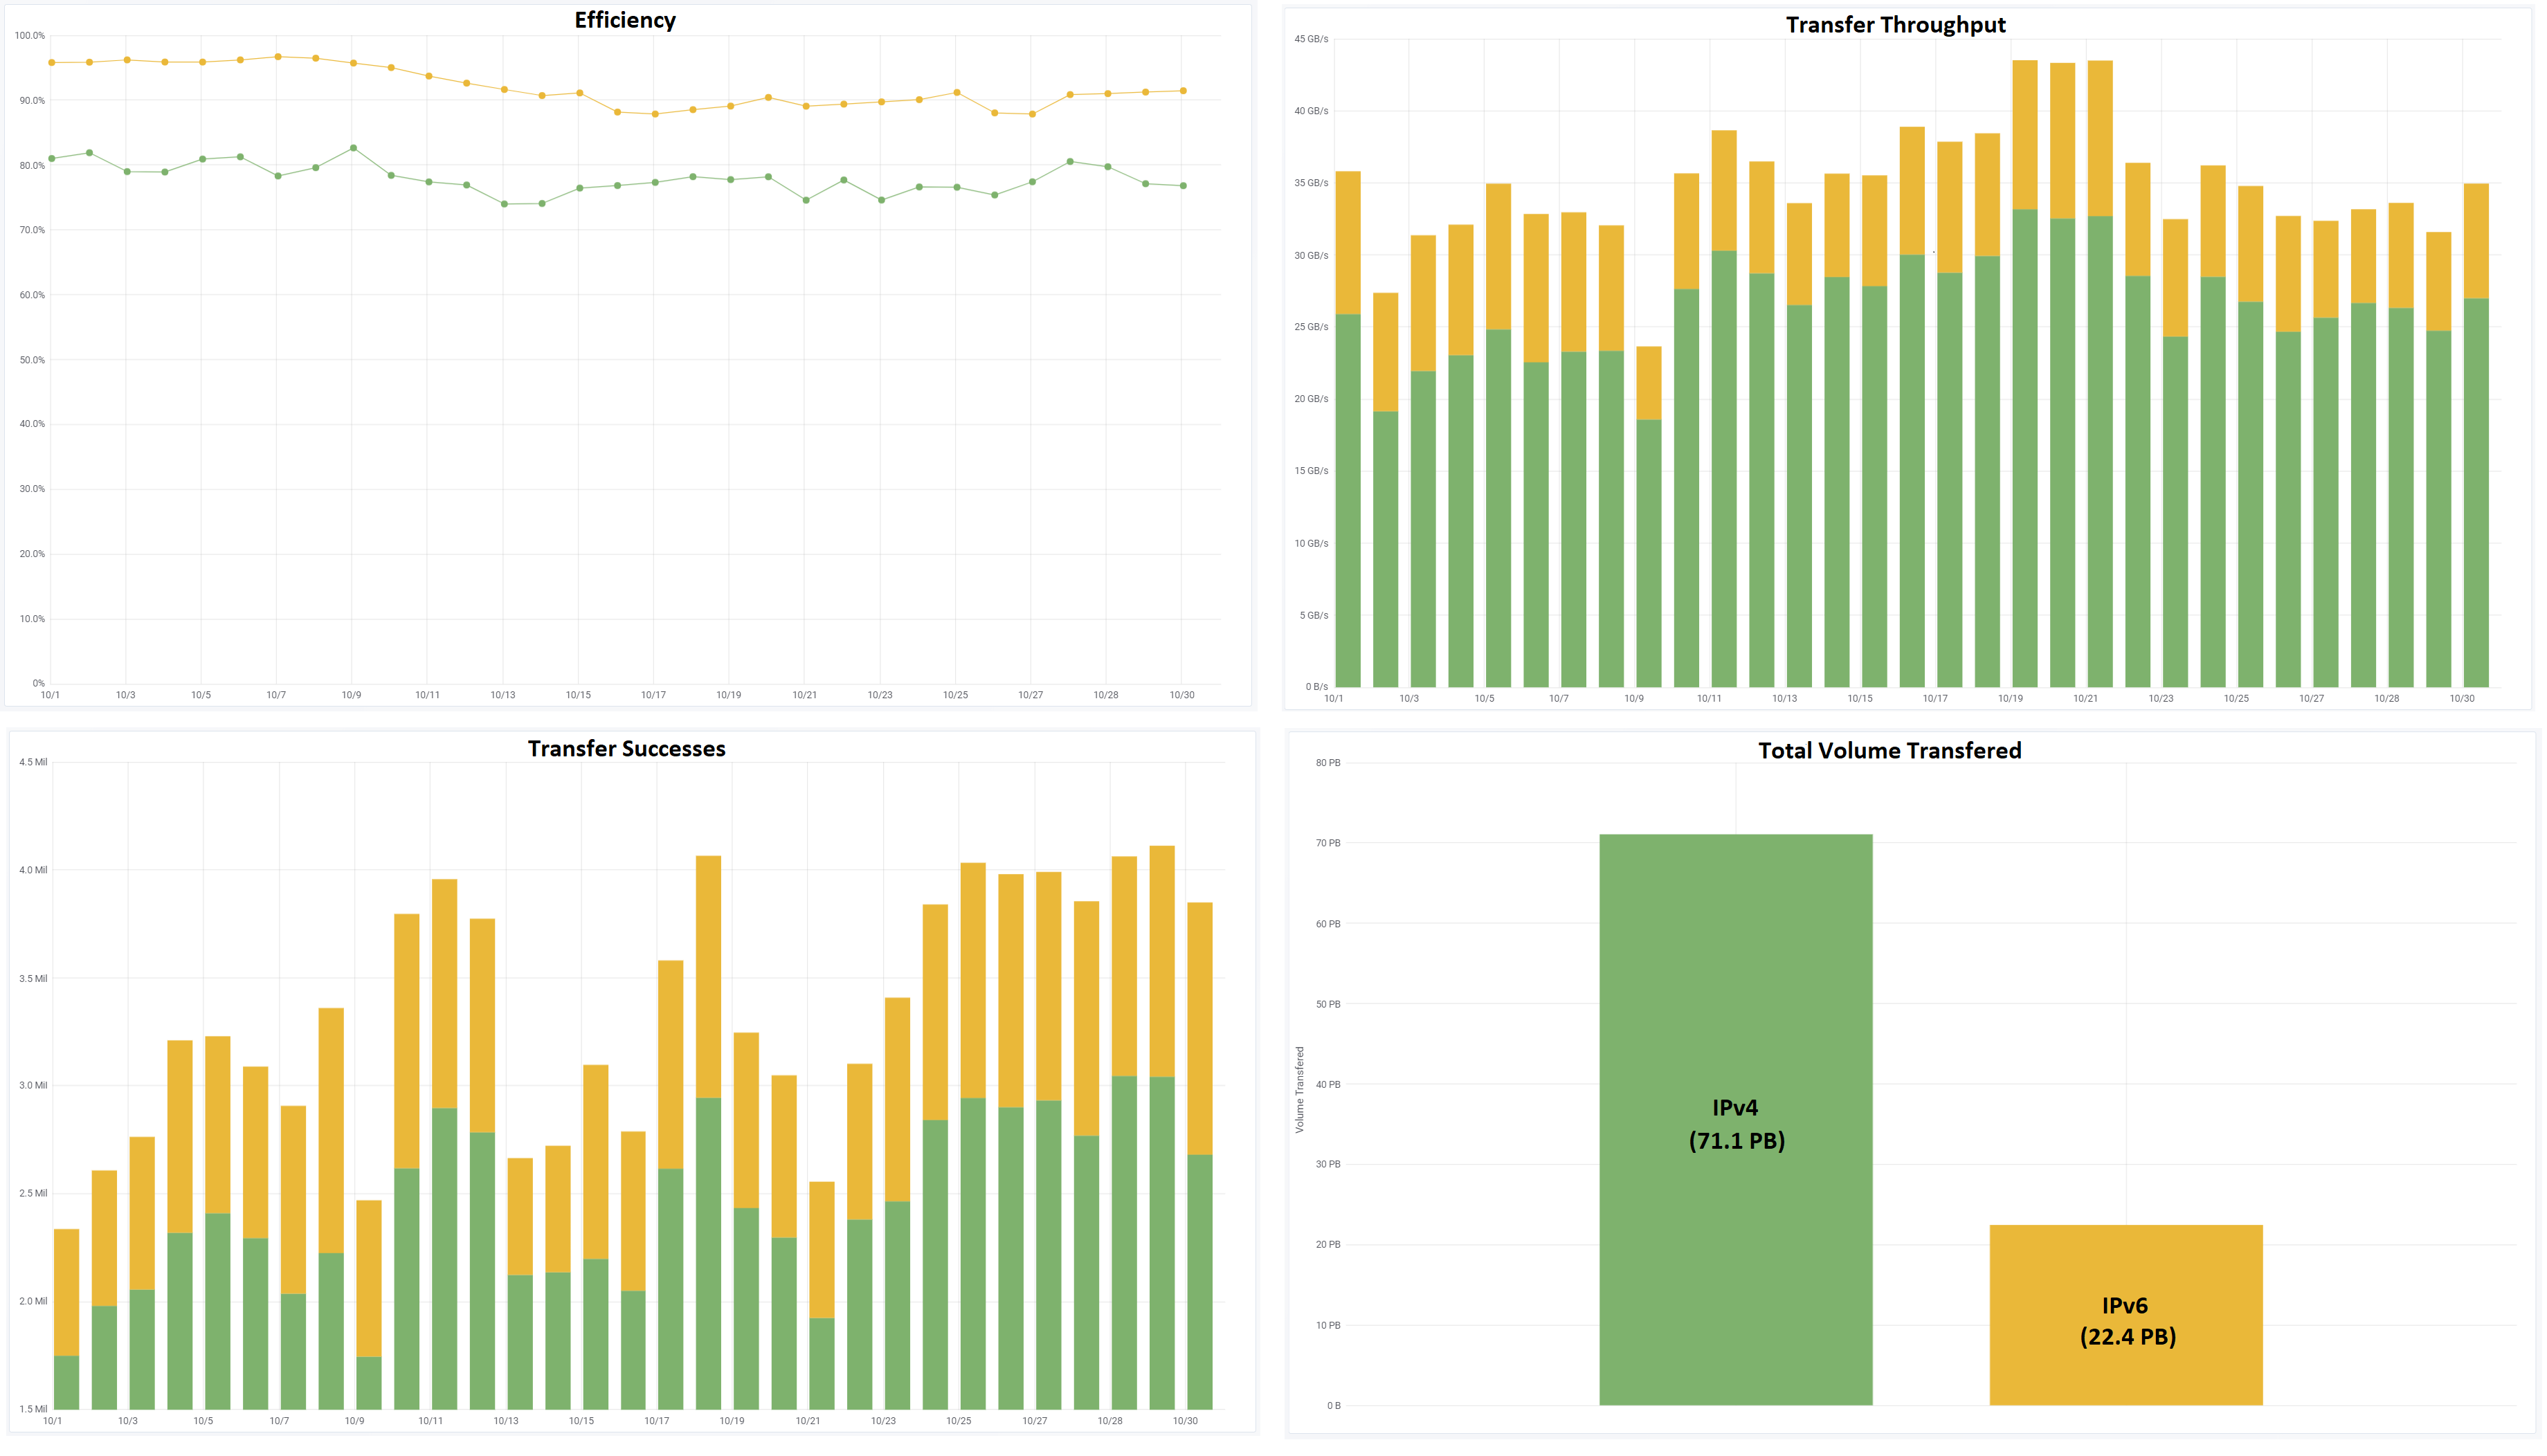
\includegraphics[width=13cm]{FTS-IPv6-figure}
%\includegraphics[width=13cm]{fts1}
%\includegraphics[width=13cm]{fts2}
\caption{FTS transfer throughput for Oct 2018 and success rate according to whether IPv6 was used. IPv4 is green; IPv6 is amber}
\label{fig:fts}
\end{figure}

\subsection{XrootD}
The other major method by which data is accessed, often remotely, is XrootD most notably by the ALICE and CMS experiments. Currently, the Monit WLCG Transfers Monitoring Service at CERN \cite{grafana-WLCG-Transfers} does not display whether this data was transferred over IPv4 or IPv6. However, the XrootD monitoring data has now been updated to report whether IPv4 or IPv6 was used \cite{xrootd-ipv6} and work is in progress to include this information in the Monit monitoring.


